\chapter[RMQ]{Range Minimum Query}
\writer{Felix Lauenroth \& Michael Mardaus}

\section{Einleitung}

Im Folgenden besch�ftigen wir uns mit dem $Range~ Minimum~  Query~ (RMQ)$ Algroithmus und dem Skyline Problem. In Kapitel 1 er�rtern wir zun�chst den $RMQ$ und zeigen verschiedene Implementationen. Kapitel 2 behandelt das Skyline Problem und zeigt unsere Umsetzung.

\section{Definition}

 Kommen wir zun�chst zur Definition der $ RMQ $. Als Eingabe wird ein Array genutzt, innerhalb welchem wird die Indexposition des kleinsten Wertes eines gegebenen Intervall's [l, r] suchen oder mathematisch Ausgedr�ckt:

\[\text{RMQ}_{A}(\ell,r) = \text{arg} \ \min_{\ell \leq k \leq r } A[k] \]

\section{Naive Ans�tze}
\subsection{Durch iterieren}

Zun�chst beschreiben wir eine auf den ersten Blick einfach aussehende Methode. Wir iterieren sequenziell durch das gegebene Intervall und speichern dabei die Indexposition des Minimums. Dies schaffen wir offensichtlich in $\Oh(n)$ \footnote{\label{foot:1} $n$ beschreibt die L�nge des Intervalls}. Wie auf den ersten Blick erkennbar ist variiert die Laufzeit mit der L�nge des gegebenen Intervalls. Auch bei mehrfach Ausf�hrung der Abfrage verschlechtert sich die Laufzeit um den erheblichen Faktor $m$\footnote{\label{foot:2} $m$ beschreibt die Anzahl der Abfragen}, welches zu einer Laufzeit von $\Oh(n\cdot m)$ bei $m$ Abfragen f�hrt. Doch diese Methode hat auch einen erheblichen Vorteil. Sie funktioniert in-place, das hei�t sie ben�tigt nur eine konstante Menge an Speicher. Denn das durch-iterieren findet in der Eingabeliste statt und ansonsten wird nur Speicherplatz f�r die Indexposition ben�tigt.

\subsection{Preprocessing}

\subsection{Preprocessing mit dynamischer Programmierung}

\section{Effiziente Algorithmen}
\subsection{$\sqrt n $ Teile Algorithmus}

\subsection{Sparse Table}
Als n�chstes er�rtern wir den Sparse Table Algorithmus ($STA$). Der $STA$ besteht im Wesentlichen aus zwei Phasen. In Phase 1 wird zun�chst eine Matrix $A$ mit $n$ Zeilen und $\lfloor \log n \rfloor +1$ Spalten erstellt. Der ein oder andere Leser wird sich jetzt fragen, wieso brauchen wir nur $\lfloor \log n \rfloor +1$ Spalten? Dies l�sst sich am besten anhand eines Beispiels zeigen. Angenommen wir haben folgendes Eingabearray (Abb. \ref{sparse_0}) .
\begin{figure}[h]
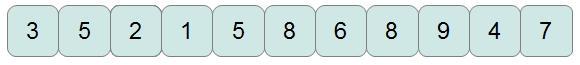
\includegraphics[width=6cm]{picture/sparse_0.png}
\caption{Eingabearray}
\label{sparse_0}
\end{figure}
Zun�chst ben�tigen wir die Zweierpotenz, welche mindestens die H�lfte des Arrays �berdeckt. In unserem Beispiel ist es die 8. Jetzt kommen wir zu dem Trick, und zwar benutzen wir nun die Tatsache das wenn wir zweimal diese Zweierpotenz benutzen, wir das Array komplett �berdecken k�nnen (Abb. \ref{sparse_01}).
\begin{figure}[h]
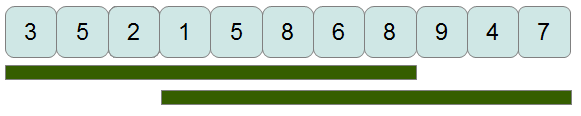
\includegraphics[width=6cm]{picture/sparse_01.png}
\caption{�berdeckung}
\label{sparse_01}
\end{figure}
Dadurch k�nnen wir das Minimum des Arrays ermitteln, indem wir jeweils das Minimum der beiden Zweierpotenzen bestimmen und davon einfach den kleineren Wert benutzen.
Diesen Trick benutzen wir nun um unsere Matrix $A$ aufzubauen. Im Wesentlich baut sich $A$ folgenderma�en auf. Jede Zeile steht f�r die entsprechende Position im Array und die Spalten entsprechen einer Zweierpotenz (Abb. \ref{sparse_02} und \ref{sparse_03}).
\begin{figure}[h]
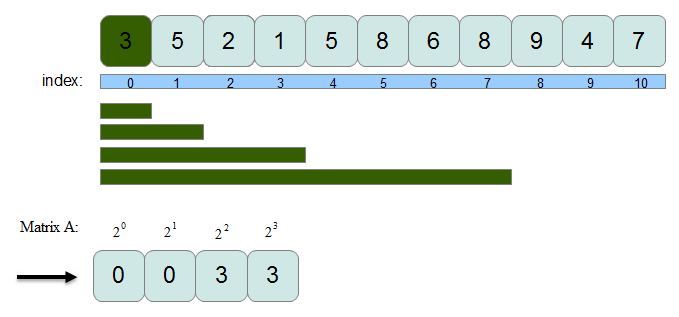
\includegraphics[width=10cm]{picture/sparse_02.png}
\caption{Erste Zeile Matrix $A$}
\label{sparse_02}
\end{figure}
\begin{figure}[h]
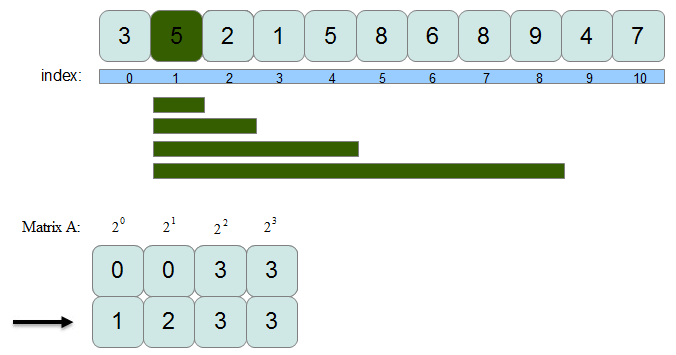
\includegraphics[width=10cm]{picture/sparse_03.png}
\caption{Zweite Zeile Matrix $A$}
\label{sparse_03}
\end{figure}
Dies f�hren wir f�r jede Position im Array durch. Nun haben wir unseren 'Sparse Table'\footnote{\label{sparse:1} sparse, da unsere Matrix $A$ nur $\lfloor \log n \rfloor +1$ Spalten besitzt, und nicht $n$ Spalten} erstellt und haben damit Phase 1 abgeschlossen. Anzumerken ist noch das die Initialisierung der Matrix $A$ durch dynamische Programmierung optimiert werden kann. Dazu wird beim Berechnen der Zeilen nicht f�r jede Spalte das Array komplett durchlaufen, sondern nur noch der Teil des Array der noch nicht besucht wurde.
Kommen wir nun zur Phase 2. Hierbei benutzen wir nun das Intervall innerhalb unseres Arrays in welchem wir das Minimum suchen. Dazu gehen wir wie folgt vor, zun�chst suchen wir die Zweierpotenz welche mindestens die H�lfte des Intervalls �berdeckt. Auch hier werden wir das Ganze durch ein einfaches Beispiel erl�utern.
Zun�chst sei unser Intervall zwischen Index 1 und 9 gegeben. Das hei�t unsere Zweierpotenz ist hier 8. Nun brauchen wir nur noch in den beiden entsprechenden Zeile unserer Matrix $A$ an Position 3\footnote{\label{sparse:2} da $2^3$ = 8} (Abb. \ref{sparse_04}).
\begin{figure}[h]
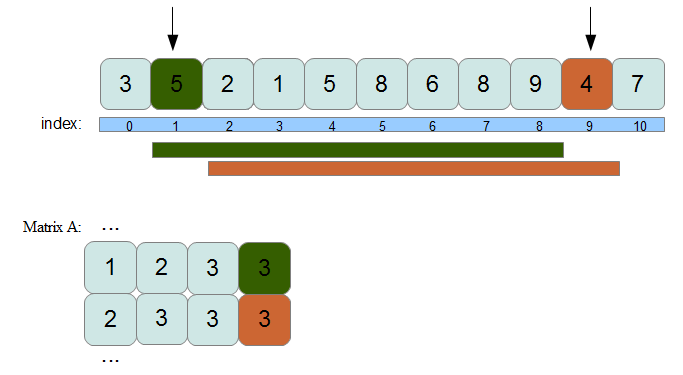
\includegraphics[width=10cm]{picture/sparse_04.png}
\caption{Abfrage}
\label{sparse_04}
\end{figure}
nachsehen und von den beiden Positionen das Minimum zu bestimmen. \\
Kommen wir nun zur Laufzeit Analyse. Offensichtlich ben�tigen wir f�r Phase 1 $\Oh(n \cdot \log n )$ um unsere Matrix $A$ zu berechnen. F�r eine Minimumbestimmung hingegen ben�tigen wir nur zwei Abfragen unserer Matrix $A$ welches wir in $\Oh 1$ schaffen. Daraus ergibt sich eine Laufzeit bei $m$ Abfragen von $\Oh (n \cdot \log n \cdot m)$.

\chapter{Skyline}

\section{Problemstellung}

\section{Anhang}
